\ifx \globalmark \undefined %% This is default.
	\documentclass[twoside,openright,11pt,a4paper]{report}

%\compiler avec xelatex
%\usepackage[applemac]{inputenc}
\usepackage[T1]{fontenc}
\usepackage[utf8]{inputenc} %latin1 est possible
%\usepackage[latin1]{inputenc} %latin1 est possible
\usepackage[UKenglish]{babel}
\usepackage{lettrine}

%\usepackage[text={13cm,20cm},centering]{geometry}
\usepackage [squaren, Gray, mediumqspace]{SIunits}
\usepackage [top=2cm, bottom=2cm, left=2cm, right=2cm ]{geometry}

\renewcommand{\familydefault}{cmss}
\addto\captionsenglish{ \renewcommand\chaptername{Solutions of Chapte}}

\usepackage{graphicx}
\usepackage{amsmath}
\usepackage{amsfonts}
\usepackage{amssymb}
\usepackage{amsthm}
\usepackage{bm}
\usepackage{color}

\newcommand{\real}{\mathbb{R}}
\newcommand{\mb}{\mathbf}
\newcommand{\bos}{\boldsymbol}

\def \RR {I \! \! R}

\newcommand{\e}{\begin{equation}}  
\newcommand{\ee}{\end{equation}}
\newcommand{\eqn}{\begin{eqnarray}} 
\newcommand{\eeqn}{\end{eqnarray}} 
\newcommand{\eqnn}{\begin{eqnarray*}} 
\newcommand{\eeqnn}{\end{eqnarray*}} 

\newcommand{\bpm}{\begin{pmatrix}}
\newcommand{\epm}{\end{pmatrix}}

%\newcommand{\{\c c}}{\c c}

\newcommand{\bma}{\left(\begin{array}}
\newcommand{\ema}{\end{array}\right)} 
\newcommand{\hh}{\hspace{2mm}}
\newcommand{\hd}{\hspace{5mm}}
\newcommand{\hu}{\hspace{1cm}}
\newcommand{\vv}{\vspace{2mm}}
\newcommand{\vd}{\vspace{5mm}}
\newcommand{\vm}{\vspace{-2mm}}
\newcommand{\teq}{\triangleq}
%\newcommand{\qedb}{\,$\Box$}
\newcommand{\blanc}{$\left. \right.$}
\newcommand{\frts}[2]%
         {\frac{{\textstyle #1}}{{\textstyle #2}}}

\newcommand{\bindex}[3]%
{
\renewcommand{\arraystretch}{0.5}
\begin{array}[t]{c}
#1\\
{\scriptstyle #2}\\
{\scriptstyle #3}
\end{array}
\renewcommand{\arraystretch}{1}
}

\theoremstyle{definition}
\newtheorem{exemple}{{\bf Exemple}}[chapter]
\newtheorem{theoreme}[exemple]{{\bf Th{é}or{è}me}}
\newtheorem{propriete}[exemple]{{\bf Propri{é}t{é}}}
\newtheorem{definition}[exemple]{{\bf D{é}finition}}
\newtheorem{remarque}[exemple]{{\bf Remarque}}
\newtheorem{remarques}[exemple]{{\bf Remarques}}
\newtheorem{lemme}[exemple]{{\bf Lemme}}
\newtheorem{hypothese}[exemple]{{\bf Hypoth{è}se}}
\newtheorem{exercice}{{\bf Exercice}}[chapter]

\newcommand{\xqedhere}[2]{%
 \rlap{\hbox to#1{\hfil\llap{\ensuremath{#2}}}}}

\newcommand{\xqed}[1]{%
 \leavevmode\unskip\penalty9999 \hbox{}\nobreak\hfill
 \quad\hbox{\ensuremath{#1}}}

\newcommand{\gf}{\fg\,\,}

\newcommand{\cata}[1] %
     {\renewcommand{\arraystretch}{0.5}
     \begin{array}[t]{c} \longrightarrow \\ {#1} \end{array}
     \renewcommand{\arraystretch}{1}}

\usepackage[isu]{caption}
%\usepackage[font=small,format=plain,labelfont=bf,up,textfont=it,up]{caption}
\setlength{\captionmargin}{60pt}

\newcommand{\cqfd}
{%
\mbox{}%
\nolinebreak%
\hfill%
\rule{2mm}{2mm}%
\medbreak%
\par%
}

\pagestyle{headings}

\renewcommand{\sectionmark}[1]{%
\markright{\thesection.\ #1}{}}

\renewcommand{\chaptermark}[1]{%
\markboth{\chaptername\ \thechapter.\ #1}{}}

\makeatletter 
\def\@seccntformat#1{\csname the#1\endcsname.\;} 
\makeatother

\title{ {\Huge {\textbf{Modélisation et analyse  \\ \vspace{4mm} des systèmes dynamiques }}} \\ \vspace{4cm} G. Bastin}

%\title{ {\Huge {\textbf{Modelisation et analyse  \\ \vspace{4mm} des systemes dynamiques }}} \\ \vspace{4cm} G. Bastin}


\date{\today}
	\begin{document} %% Crashes if put after (one of the many mysteries of LaTeX?).
\else 
	\documentclass{standalone}
	\begin{document}
\fi

\graphicspath{ {Chapitre2/images/} }


\setcounter{chapter}{1}
\chapter{Articulated mechanical systems}
\chaptermark{Articulated mechanical systems}\label{systmeca}




\lettrine[lines=1]{\bf T}{}he subject of this chapter is setting in equations state models of mechanical systems formed of a set of rigid bodies connected by joints. The systematic modeling method that we will study is applicable to many practical examples of mechanical systems such as vehicles (cars, trains, planes, ...) or robots. This method results from a systematic application of Newton's law.

In order to simplify the notations and calculations, we will limit ourselves to the establishment of the motion equations in a two-dimensional space
(i.e. in a plane). The extension to the case of a movement in a three-dimensional space is conceptually simple but more difficult to visualize.

We first consider the case of a single rigid body without friction. Then, we discuss the modeling of an articulated system consisting of several rigid bodies. The modeling method is described in detail using an example of a \blue{robot manipulator} with two degrees of freedom. Finally, we discuss how to extend the model to take into account friction, the elasticity of the joints and the non-holonomic constraints.

\section{Dynamics of a rigid body in the plane}

We consider a rigid body moving in a plane in which an orthonormal inertial basis $ 0,X_B, Y_b$ is fixed arbitrarily (Fig.\ref{Fig:corigidplan}).
\begin{figure}[h]
\begin{center}
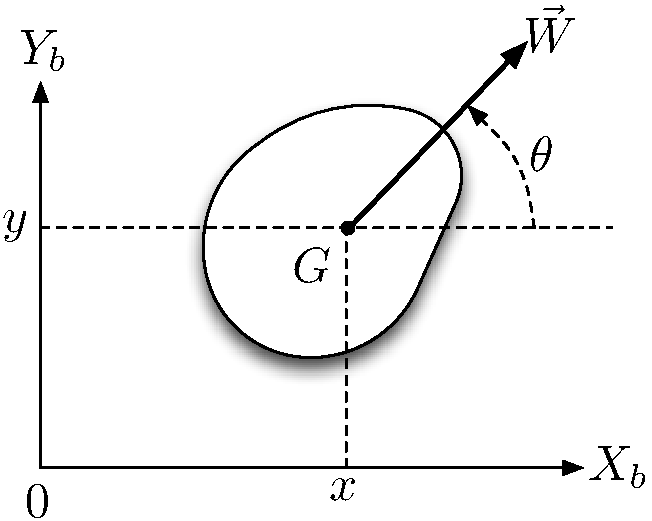
\includegraphics[width=6cm]{corigidplan}
\caption{Coordinates of a rigid body in plane}
\label{Fig:corigidplan}
\end{center}
\end{figure}
A vector $\vec{W}$ is attached to the body. The position of the body is completely specified by the 3 coordinates $x, y, \theta$: 
\begin{itemize}
\item $x, y$ are the Cartesian coordinates of the center of mass $G$ in the fixed basis $0,X_b,Y_b$~;
\item $\theta$ is the orientation of the vector $\vec{W}$ with respect to the fixed basis $0,X_b,Y_b$. 
\end{itemize}
We define the three-dimensional vector describing the position of the body:
\eqn
q \triangleq \bma{c} x \\y \\ \theta \ema. \label{cogen}
\eeqn

\noindent A direct application of Newton's laws, coordinate by coordinate, then leads to the following general equations of motion:
\begin{itemize}
\item Equations of translation of the center of mass :
\eqnn
m\ddot{x} &=& F_x, \\ m\ddot{y} &=& F_y.
\eeqnn
\item Equation of rotation around the center of mass :
\eqnn
I\ddot{\theta} = T.
\eeqnn
\end{itemize}

\noindent where $m$ is the mass of the body, $I$ is its moment of inertia with respect to the center
mass,
$F_x$ and
$F_y$ denotes the projections of the resultant of the forces applied to the body on the
axes $0X_b$ and $0Y_b$ 
respectively and $T$ is the resultant of the torques applied
for the rotation of the body around the center of mass.

These general equations of motion form the basis of the establishment
of the system state model as we will illustrate it in an example.

\begin{exemple}{\bf Modeling of the dynamics of a rocket.}

We consider a rocket moving in a plane perpendicular to the ground. This rocket is propelled by two jet engines arranged symmetrically with respect to the body of the rocket as shown in Figure \ref{Fig:fusee}. 
\begin{figure}[ht]
\begin{center}
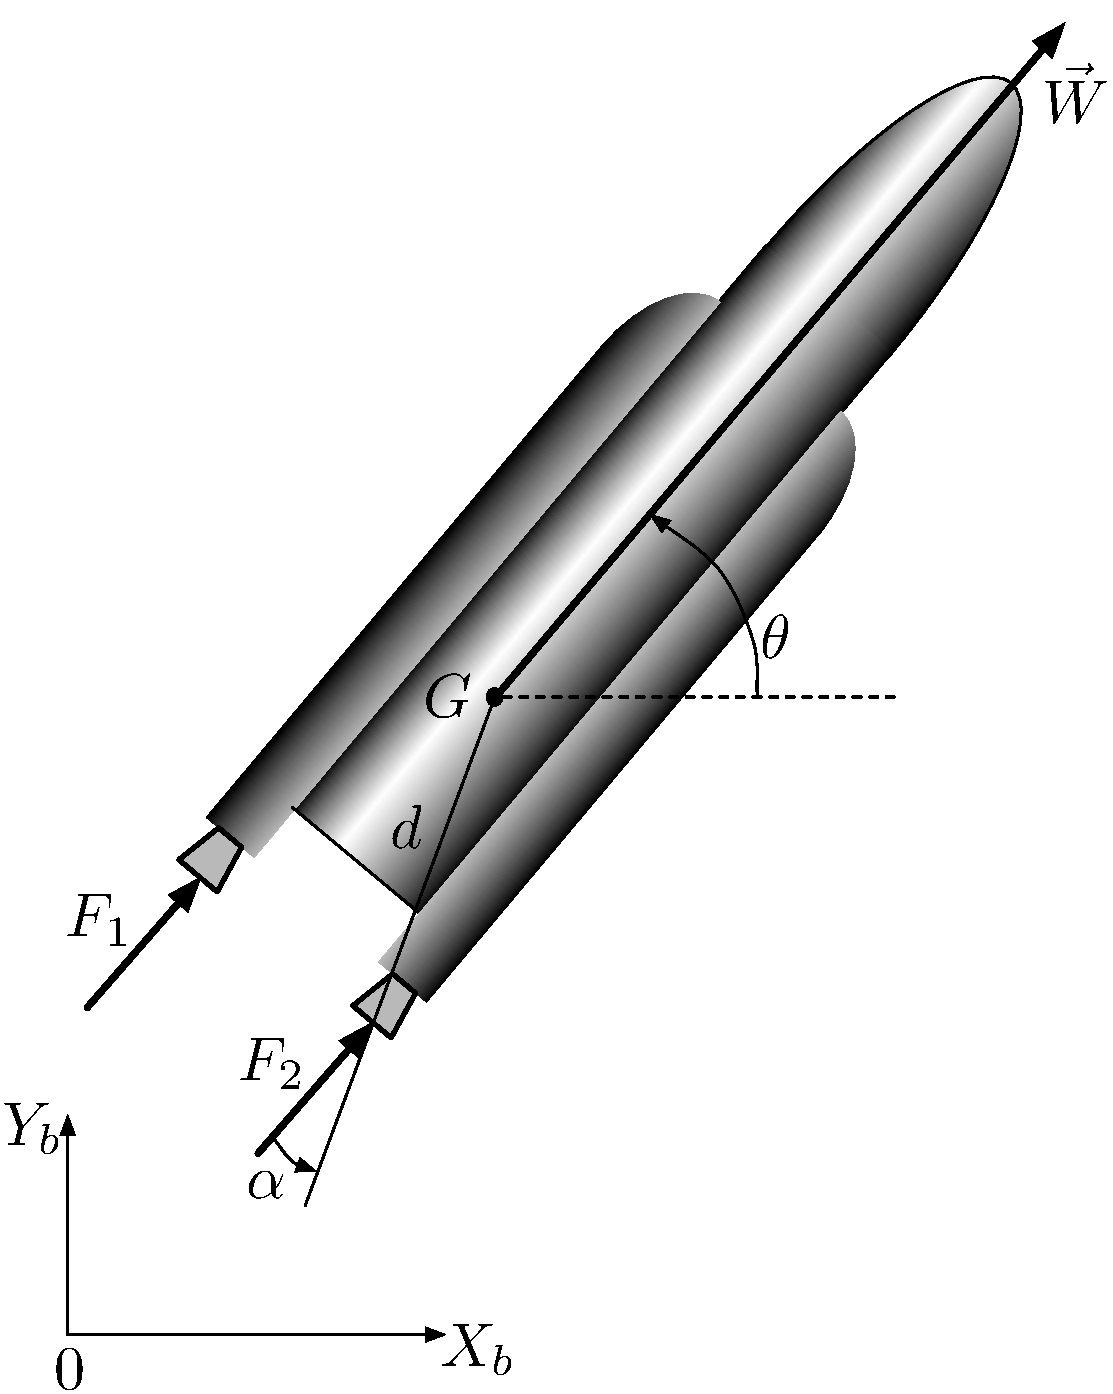
\includegraphics[width=8cm]{fusee}\hfill
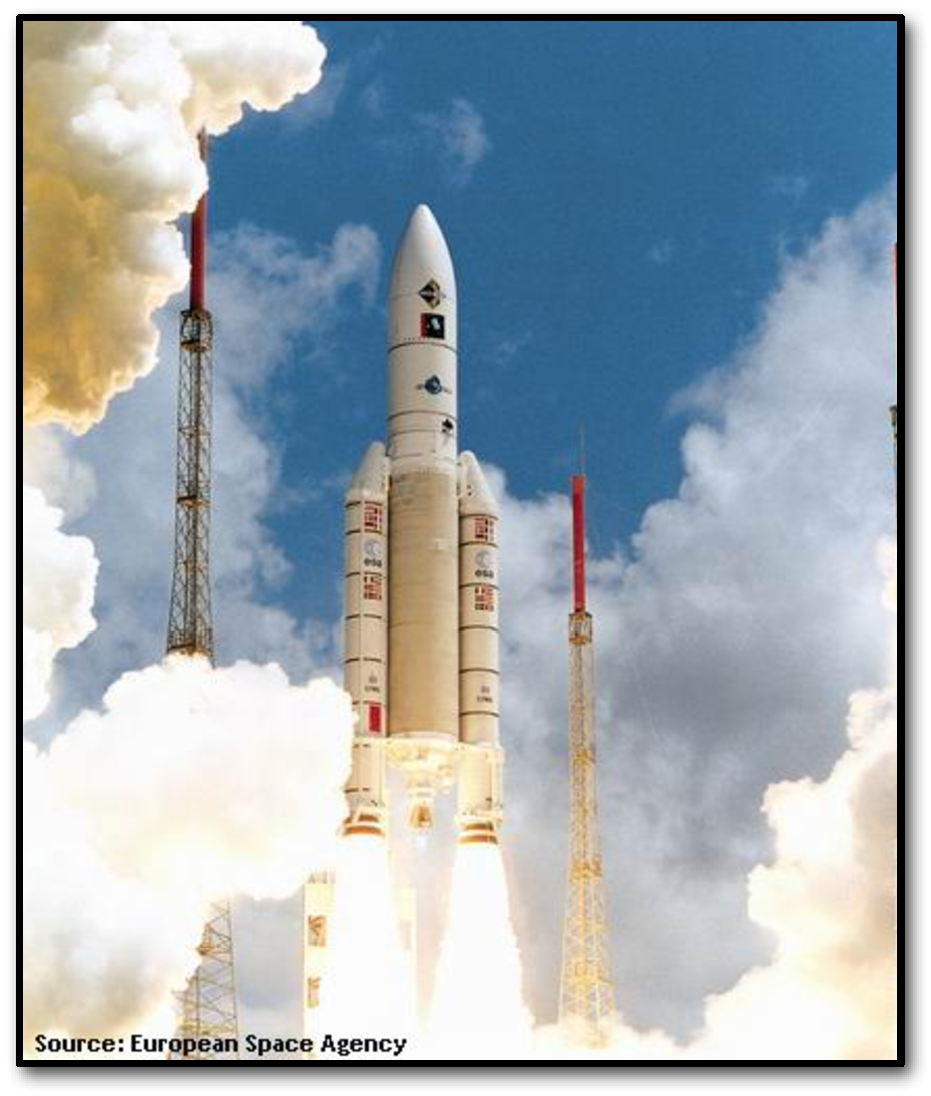
\includegraphics[width=4.6cm]{ariane}
\caption{Modeling of the dynamics of a rocket - Photo of the Ariane rocket during takeoff (\copyright \,ESA)}
\label{Fig:fusee}
\end{center}
\end{figure}
The equations of motion are established under  {\bf the modeling assumption} that the rocket is a rigid body of constant mass.
\begin{itemize}
\item Equations of translation :
\begin{equation} \begin{split} \label{transfus}
m\ddot{x} &= F_x = (F_1 + F_2)\cos\theta, \\ 
m\ddot{y} &= F_y = (F_1 + F_2)\sin\theta - mg_0.  
\end{split} \end{equation}
\item Equation of rotation :
\eqn
I\ddot{\theta} = T = (F_2 - F_1)d\sin\alpha. \label{rotfus}
\eeqn
\end{itemize}
\noindent 
In these equations, $(x, y)$ is the position of the center of mass $G$, $\theta$ the angle of the vector $\vec W$ with respect to the horizontal, $F_ {1}, F_ {2}$ \blue{the thrusts of the reactors}, $m$ the mass of the rocket, $I$ its moment of inertia, $d, \alpha$ geometrical parameters (Fig.\ref{Fig:fusee}) and $g_0$ the gravitational constant.

The equations (\ref{transfus})-(\ref{rotfus}) can be put in the standard form of a state model $\dot{x} =
f(x,u)$ of dimension 6 with two inputs if we introduce the following notations~:
\begin{description}
\item {\em State variables:}
\eqnn
x_1 = x, \hspace{6mm} x_2 = y, \hspace{6mm} x_3 = \theta, \hspace{6mm} x_4 = \dot{x}, \hspace{6mm} 
x_5 = \dot{y}, \hspace{6mm} x_6 = \dot{\theta}.
\eeqnn
\item {\em Input variables :}
\eqnn
u_1 = F_1, \hspace{10mm} u_2 = F_2.
\eeqnn
\end{description}
The state model is written as follows~:
\begin{equation*} \begin{split}
\dot x_1 &= x_4, \\
\dot x_2 &= x_5, \\
\dot x_3 &= x_6, \\
\dot x_4 &= \frac{\cos x_3}{m} (u_1 + u_2), \\
\dot x_5 &= - g_0 + \frac{\sin x_3}{m} (u_1 + u_2), \\
\dot x_6 &= \frac{d \sin \alpha }{I} (u_2 - u_1). \qed
\end{split} \end{equation*}
\end{exemple}

A special situation appears when the considered body is subject to a set of forces whose resultant is zero but which are not all applied at the same point. The equations of motion can be written as :
\eqnn
m\ddot{x} &=& 0\\ 
m\ddot{y} &=& 0 \\
I\ddot{\theta} &=& T 
\eeqnn
In such a case, it is common, in some applications, to not specify the forces that are behind the torque $T$, but to directly consider this one as the cause of the movement. We say, for simplicity, that the body is subjected to a {\em torque}. Thus, for example, we will talk about the torque provided by an engine to rotate a \blue{robot manipulator} segment.

The state model obtained in the example of the rocket is non-linear with respect to the state variables and affine in the input variables. This will be the case for most applications of interest for which the translational and rotational equations describing the dynamics of a rigid body can be written in the general matrix form :
\eqnn
J\ddot{q} + b(q) = B(q)u.
\eeqnn
In this equation $J$ is the inertia matrix (diagonal and constant), $b(q)$
represents the effect of gravity and 
$B(q)$ is a
matrix (called kinematic) non-linearly depending on the state variables. 
We deduce that the state model is written in the following general form :
\eqnn
\dot{q} &=& v, \\ 
\dot{v} &=& J^{-1}[-b(q) + B(q)u],
\eeqnn
where $v \triangleq \dot{q}$ is called {\em vector of generalized velocities}.

\section{Dynamics of articulated mechanical systems}

We now consider the case of an articulated mechanical system with N body. The general procedure for setting in equations the state model can be summarized as follows~:
\begin{enumerate}
\item Fix an inertial reference frame in the system configuration space and $N$ moving frames attached to the centers of mass of the $N$ bodies of the system.
\item Write the \blue{path and bonding constraints} equations faced by the movement of the system. Deduce the number of degrees of freedom.
\item Write the equations of motion (translation and rotation) for each of the coordinates by including the bonding forces related to the constraints (method of Lagrange coefficients).
\item Remove the coefficients of Lagrange and redundant coordinates.
\end{enumerate}

We will now detail the procedure, explaining the new concepts (degrees of freedom, Lagrange coefficients, redundant coordinates) that have been mentioned, and illustrate it with a typical example: the development of the dynamic model of a \blue{robot manipulator} with two degrees of freedom.

\vspace{5mm}

\noindent {\bf First step: Defining coordinate}

An inertial reference frame is set in the configuration space $\Omega$ of the system. $N$ moving frames are attached to the centers of mass of the $N$ bodies of the system. The position of the system is at any time characterized by the coordinate vector
\eqnn
\xi = (x_1 \; y_1 \; \theta_1 \; . \; . \; .\; x_N\; y_N\; \theta_N)^{T}
\eeqnn
of dimension $3N$.

\vspace{5mm}

\noindent {\bf Step Two: Expression of geometric constraints}

The movement of an articulated mechanical system may be subject to two types of constraints (called geometric) : \blue{path contraints} on the one hand and bonding contraints between the bodies on the other hand. These constraints are expressed as a set of algebraic relations between the coordinates which we will note
\eqnn
\Psi (\xi) = 0,
\eeqnn
where $\Psi$ is an application $\Omega \rightarrow \RR^p$ of class $C^1$ and $p$
denotes the number of constraints. According to the implicit function theorem, in a neighborhood of any point $\xi$
of the configuration space, there is a partition $\xi = (q, \bar{q})$ of the coordinates vector such that :
\begin{itemize}
\item the dimension (noted $\sigma$) of $\bar{q}$ is equal to the rank of the Jacobian matrix of the application $\Psi$ :
\eqnn
\sigma \triangleq \mbox{dim}\bar{q} = \mbox{rank}\frac{\partial \Psi}{\partial \xi};
\eeqnn
\item we can express the coordinates $\bar{q}$ depending on coordinates $q$ :
\eqn
\bar{q} = \phi (q) \label{red}.
\eeqn
\end{itemize}
\noindent This means that we can use the expression (\ref{red}) to remove the {\em redundant coordinates} $\bar q$ of the system description. The size of the vector $q$ of the coordinates that are preserved is the {\em number of degrees of freedom} of the system, denoted $\delta$ :
\eqnn
\delta \triangleq 3N - \sigma.
\eeqnn

\vspace {5mm}

\noindent {\bf Step Three: Equations of motion}

Then we write the equations of motion (translation and rotation) for each of the coordinates by including the bonding forces related to the constraints. The partition $(q,\bar{q})$ of the coordinates induces a similar partition of the set of equations of motion as follows :
\eqn
J\ddot{q} + b(q,\bar{q}) &=&  B(q,\bar{q})u + w, \label{mo1}\\[2mm]
\bar{J}\ddot{\bar{q}} + \bar{b}(q,\bar{q}) &=& \bar{B}(q,\bar{q})u + \bar{w}. \label{mo2}
\eeqn
In these equations, vectors $w$ and  $\bar{w}$ represent the bonding forces that ensure that the constraints are satisfied at any time during the movement of the system. It is shown in the mechanical basic works that these binding forces are expressed as follows :
\eqnn
w &=& - A(q)\lambda, \\
\bar{w} &=& \lambda.
\eeqnn
where $\lambda$ is the vector of {\em Lagrange coefficients} (of dimension $\sigma$)
and $A(q)$ is the matrix of dimension $\delta \times \sigma$ defined as follows :
\eqnn
A(q) \triangleq (\frac{\partial \phi}{\partial q})^{T}.
\eeqnn

\vspace{5mm}

\noindent {\bf Step Four: Eliminate redundant coordinates}

In the equation (\ref{mo2}), $\lambda$ is expressed as :
\eqnn
\lambda = \bar{J}\ddot{\bar{q}} + \bar{b}(q,\bar{q}) - \bar{B}(q,\bar{q})u.
\eeqnn
En substituant cette expression dans (\ref{mo1}) et en utilisant (\ref{red}), on obtient :
\begin{equation} \begin{split}
J\ddot{q} + A(q)\bar{J}\ddot{\bar{q}} &+ b(q,\phi(q)) + A(q)\bar{b}(q,\phi(q)) \\
&= (B(q,\phi(q)) + A(q)\bar{B}(q,\phi(q)))u \label{g1}.
\end{split} \end{equation}
Il ne reste plus alors qu'à éliminer $\ddot {\bar q}$. Pour cela on différencie deux
fois l'expression (\ref{red}) :
\eqn
\dot {\bar q} &=& A^{T}(q)\dot q \\
\ddot {\bar q}  &=& A^{T}(q)\ddot q + \dot A^T(q)\dot q. \label{ac}
\eeqn
En substituant cette dernière expression (\ref{ac}) dans (\ref{g1}) et en introduisant les
notations suivantes :
\begin{equation*} \begin{split}
M(q) &\triangleq J + A(q)\bar{J}A^{T}(q), \\
f(q,\dot{q}) &\triangleq A(q)\bar{J}\dot{A}^{T}(q)\dot{q}, \\
g(q) &\triangleq b(q,\phi(q)) + A(q)\bar{b}(q,\phi(q)), \\
G(q) &\triangleq B(q,\phi(q)) + A(q)\bar{B}(q,\phi(q)),
\end{split} \end{equation*}
on obtient finalement le modèle dynamique général d'un système mécanique articulé 
sous la forme suivante :
\eqn
M(q)\ddot q + f(q,\dot q) + g(q) = G(q)u. \label{modmecgen}
\eeqn
\noindent Dans cette équation :
\begin{itemize}
\item $q$ est le vecteur (de dimension $\delta$) des coordonnées nécessaires 
à la description du système,
\item $M(q)$ est la matrice d'inertie (de dimensions $\delta \times \delta$) symétrique et
définie positive,
\item $f(q,\dot{q})$ est le vecteur (de dimension $\delta$) qui représente les forces et
les couples résultant des liaisons relatives aux contraintes; il peut aussi s'écrire 
sous la forme 
\eqnn
f(q,\dot{q}) = C(q,\dot{q})\dot{q}
\eeqnn
où $C(q,\dot{q})$ est la matrice de dimensions $\delta \times \delta$ définie
comme suit :
\eqnn
C(q,\dot{q}) \triangleq A(q)\bar{J}\dot{A}^{T}(q),
\eeqnn
\item $g(q)$ est un vecteur (de dimension $\delta$) représentant les forces et les
couples résultant de la gravité,
\item $u$ est le vecteur (de dimension $m$) des forces et couples appliqués au système,
\item $G(q)$ est une matrice cinématique de dimensions $\delta \times m$.
\end{itemize}

\noindent Une fois le modèle dynamique général (\ref{modmecgen}) établi, il ne reste 
qu'à en déduire le modèle d'état du système :
\begin{equation*} \begin{split}
\dot{q} &= v, \\ 
\dot{v} &= M^{-1}(q)[-f(q,v) - g(q) + G(q)u].
\end{split} \end{equation*}
Dans ces équations d'état, $q$ est le vecteur des coordonnées de position et 
$v=\dot{q}$ est le vecteur des coordonnées de vitesse.

\begin{exemple} {\bf Modèle dynamique d'un robot manipulateur.}

Un robot manipulateur est formé d'un ensemble de segments rigides 
articulés.  Les articulations sont de type roto\"\i de ou de type
prismatique.  Une articulation roto\"\i de permet un mouvement
relatif de rotation entre deux segments.  Une articulation
prismatique permet un mouvement relatif de translation entre deux
segments.

Les robots sont actionnés par des moteurs encastrés produisant
des forces de translation pour les articulations prismatiques et des
couples de rotation pour les articulations roto\"\i des.

Nous considérons le robot manipulateur représenté à la figure 
\ref{Fig:robot} et formé d'un segment rigide se déplaçant horizontalement
(corps 1) auquel est articulé un deuxième segment rigide pouvant effectuer un mouvement
de rotation (corps 2). Le mouvement du système est provoqué par la force $F$ appliquée 
horizontalement au premier segment et le couple de rotation $T$ appliqué au deuxième
segment. Le repère inertiel et les  différentes coordonnées sont indiquées sur la figure.

\begin{figure}[ht]
\begin{center}
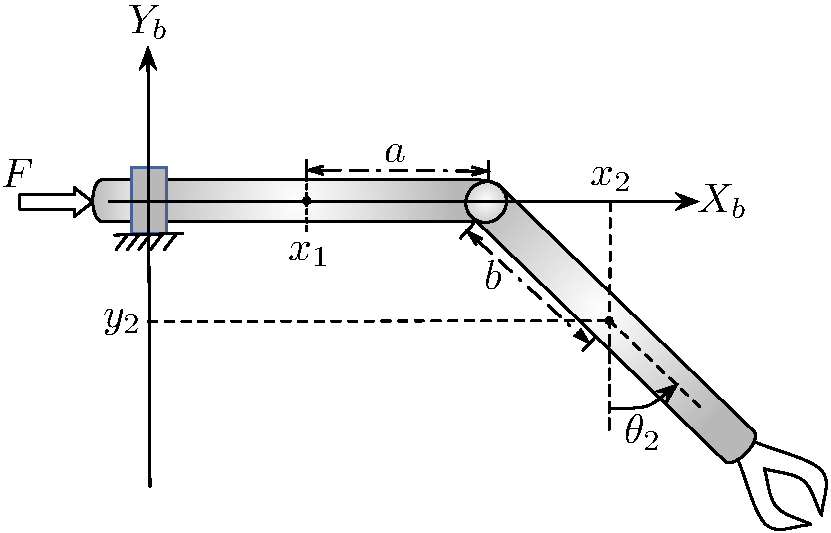
\includegraphics[width=8.5cm]{robot2}
\caption{Modélisation d'un robot manipulateur}
\label{Fig:robot}
\end{center}
\end{figure}

Ce système est soumis aux contraintes suivantes :
\begin{description}
\item {\em Contraintes de parcours :}
\begin{equation*} \begin{split}
y_1 &= 0, \\
\theta_1 &= 0.
\end{split} \end{equation*}
\item {\em Contraintes de liaison :}
\begin{equation*} \begin{split}
x_2 - b\sin\theta_2 - x_1 - a&= 0, \\
y_2 + b\cos\theta_2 &= 0.
\end{split} \end{equation*}
\end{description}
\noindent Les contraintes de parcours expriment le fait que le corps 1 ne peut se déplacer
qu'horizontalement. Les contraintes de liaison expriment la relation existant
entre les coordonnées cartésiennes des centres de masse des deux corps en raison
de leur articulation. La matrice jacobienne des contraintes s'écrit comme suit :
$$
\bma{cccccc} 0 & 1 & 0 & 0 & 0 & 0 \\ 
0 & 0 & 1 & 0 & 0 & 0\\ -1 & 0 & 0 & 1 & 0 & -b\cos\theta_2 \\
0 & 0 & 0 & 0 & 1 & -b\sin\theta_2 \ema.
$$
On observe que cette matrice est de plein rang $\sigma = 4$ et donc que le système
possède $\delta = 2$ degrés de liberté (comme on pouvait s'y attendre). On observe
aussi que l'on peut définir la partition $(q,\bar{q})$ des coordonnées comme suit:
$$
q = \bma{c} x_1 \\ \theta_2 \ema, \hh 
\bar{q} = \bma{c} y_1 \\ \theta_1 \\ x_2 \\ y_2\ema.
$$
Il est aisé de vérifier que dans tout l'espace de configuration, les coordonnées 
$\bar{q}$ peuvent s'exprimer comme une fonction explicite $\bar{q} = \phi(q)$ des 
coordonnées $q$~:
\begin{align}
y_1 &= 0, \label{c1} \\
\theta_1 &= 0, \label{c2} \\
x_2 &= x_1 + b\sin\theta_2 + a, \label{c3} \\
y_2 &= - b\cos\theta_2. \label{c4}
\end{align}
On pourra donc éliminer les coordonnées $\bar{q}=(y_1, \theta_1, x_2, y_2)^{T}$ de la
description du système et ne conserver que les coordonnées $q=(x_1, \theta_2)^{T}$.
La matrice $A(q)$ s'écrit :
$$  
A(q) = (\frac{\partial \phi}{\partial q})^{T} = \bma{cccc} 0 & 0 & 1 & 0 \\ 
0 & 0 & b\cos\theta_2 & b\sin\theta_2 \ema
$$  
Les équations du mouvement s'écrivent :
\begin{align}
m_1\ddot x_1 &= F - \lambda_3, \label{eqmo1}\\
I_2\ddot \theta_2 &= - \lambda_3b\cos\theta_2 - \lambda_4b\sin\theta_2 
+ T, \label{eqmo2} \\ 
m_1\ddot y_1 &= - m_1g_0 + \lambda_1, \label{eqmo3}\\
I_1\ddot \theta_1 &= \lambda_2, \label{eqmo4}\\
m_2\ddot x_2 &= \lambda_3, \label{eqmo5}\\
m_2\ddot y_2 &= -m_2g_0 + \lambda_4. \label{eqmo6}
\end{align}
En combinant les contraintes (\ref{c1}), (\ref{c2}) avec les équations du mouvement
(\ref{eqmo3}), (\ref{eqmo4}) on déduit les valeurs suivantes de $\lambda_1$ et $\lambda_2$ :
$$
\lambda_1 = m_1g_0,\hd \lambda_2 =0.
$$
Ces valeurs expriment les forces de liaison appliquées aux deux corps pour satisfaire
les contraintes de parcours le long du mouvement du système.

D'autre part, en éliminant $\lambda_3$ et $\lambda_4$ entre les équations du mouvement
(\ref{eqmo1}), (\ref{eqmo2}), (\ref{eqmo5}), (\ref{eqmo6}), on obtient :
\eqn
\bma{c} m_1\ddot x_1 \\ I_2\ddot \theta_2 \ema + \bma{cc} 1 & 0 \\ b\cos \theta_2
& b\sin \theta_2 \ema \bma{c} m_2\ddot x_2 \\ m_2\ddot y_2 \ema = 
\bma{c} F \\ T - bm_2g_0\sin\theta_2 \ema. \nonumber \\ \label{t1} 
\eeqn
En dérivant deux fois les contraintes (\ref{c3}), (\ref{c4}), on obtient :
\eqn
\bma{c} m_2\ddot x_2 \\ m_2 \ddot y_2 \ema = \bma{cc} 1 & b\cos\theta_2 \\ 0 & 
b\sin\theta_2 \ema \bma{c} m_2\ddot x_1 \\ m_2\ddot \theta_2 \ema + 
m_2b {\dot \theta_2}^2 \bma{c} -\sin\theta_2 \\ \cos\theta_2 \ema. \label{t2}
\eeqn
En substituant (\ref{t2}) dans (\ref{t1}), on obtient finalement le modèle du système
sous la forme désirée :
\eqn
M(q)\ddot{q} + C(q,\dot{q})\dot{q} + g(q) = G(q)u,  \label{eqmouv}
\eeqn
avec
\begin{equation*} \begin{split}
M(q) &= \bma{cc} m_1 + m_2 & m_2b\cos\theta_2 \\ m_2b\cos\theta_2 & I_2 + m_2b^2 \ema, \\
C(q,\dot{q}) &= \bma{cc} 0 & -m_2b\dot \theta_2 \sin\theta_2 \\ 0 & 0 \ema, \\
g(q) &= \bma{c} 0 \\ bm_2g_0\sin\theta_2 \ema, \\
G(q)u &= \bma{c} F \\ T \ema. \end{split} \end{equation*}
\qed

\end{exemple}

\section{Propriétés de la matrice d'inertie}

\begin{enumerate}
\item La matrice d'inertie $M(q)$ est symétrique et définie positive. En effet, elle est
la somme d'une matrice diagonale $J$ dont les éléments sont positifs et d'une
matrice symétrique et semi-définie positive $A(q)\bar{J}A^{T}(q)$.
\item La dérivée temporelle de la matrice d'inertie $\dot M(q)$ vérifie la relation suivante :
\begin{equation*} \begin{split}
\dot M(q) &= A(q)\bar{J}\dot A^{T}(q) + \dot A(q)\bar{J}A^{T}(q),  \\
&= C(q,\dot q) + C^T(q,\dot q). \label{prop2}
\end{split} \end{equation*}
Cette relation implique que la matrice
\eqn
\dot M(q) - 2C(q,\dot q) \label{prop1}
\eeqn
est antisymétrique.
\item La matrice d'inertie $M(q)$ vérifie la relation suivante :
\eqn
\frac{\partial}{\partial q}(\dot q^T M(q) \dot q) = \dot q^T C(q, \dot q). \label{prop2}
\eeqn
La vérification de cette expression est laissée à titre d'exercice.
\end{enumerate}


\section{Articulations élastiques}

Nous avons considéré jusqu'à présent des systèmes mécaniques articulés formés 
uniquement de corps rigides sans possibilité de flexibilité ou de souplesse dans les 
liaisons et les articulations. Une telle hypothèse n'est pas réaliste dans de nombreuses 
applications. Une manière simple d'introduire de la souplesse dans les articulations 
d'un système mécanique articulé est de placer un petit ressort (fictif) de masse nulle 
dans les liaisons entre corps comme indiqué sur la figure \ref{Fig:flexiart}. Ce ressort 
exerce une force de rappel sur chacun des deux corps auxquels il est attaché. Cette force 
s'applique au point de fixation du ressort et est une fonction monotone croissante de 
l'élongation du ressort. Elle s'ajoute aux autres forces appliquées au système dans 
l'écriture des équations du mouvement. Lorsque de l'élasticité est ainsi introduite 
dans une articulation entre deux corps du système, il va de soi que la ou les contraintes 
de liaison correspondantes disparaissent et que le nombre de degrés de liberté est
augmenté corrélativement. Nous illustrons la méthode sur un exemple 
simple d'un système à deux corps. 

\begin{exemple} {\bf Système à deux corps avec une articulation élastique.}

\begin{figure}[ht]
\begin{center}
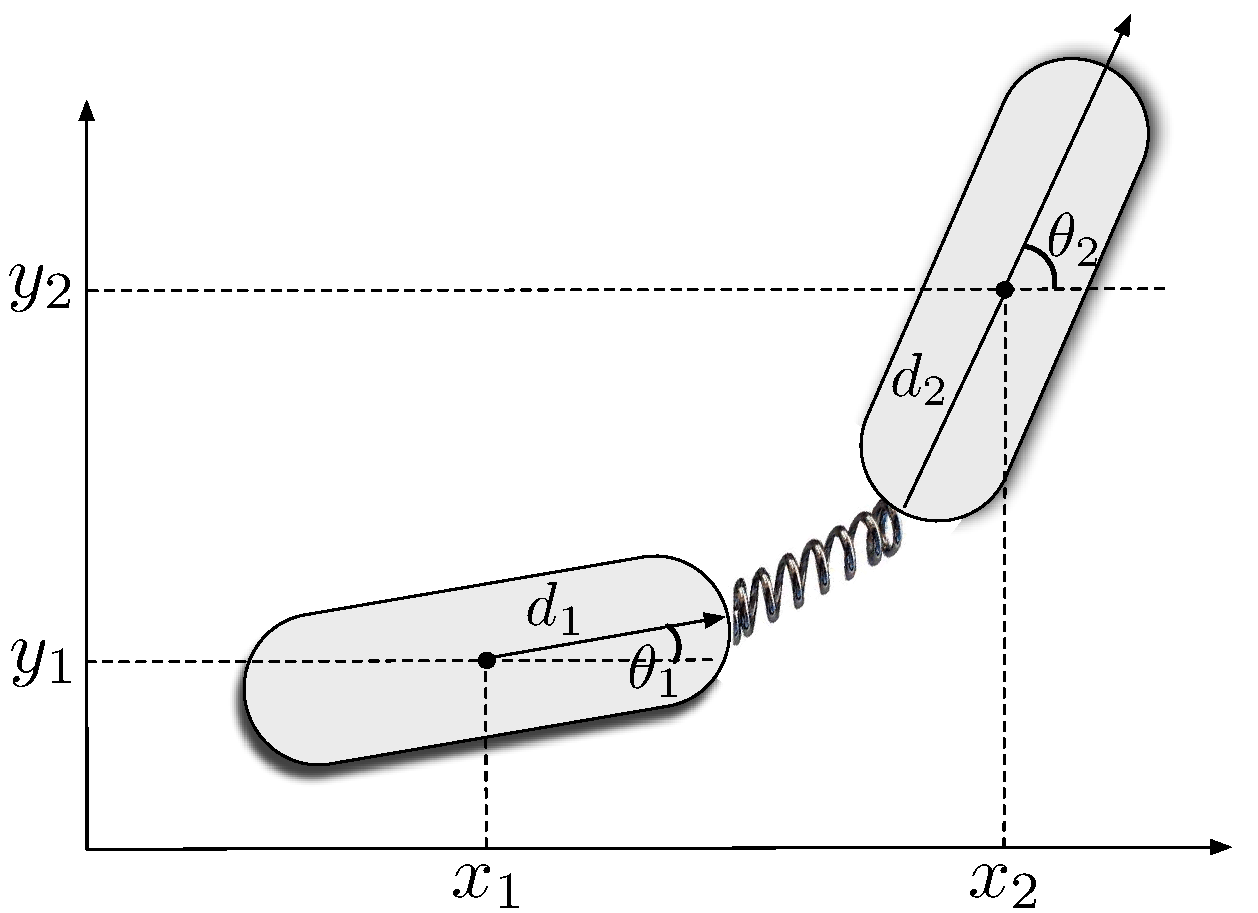
\includegraphics[width=3in]{flexiart}
\caption{Modélisation d'une articulation élastique}
\label{Fig:flexiart}
\end{center}
\end{figure}
Nous considérons le système à deux corps représenté sur la figure \ref{Fig:flexiart}.
Les équations du mouvement des deux corps s'écrivent comme suit~:
\begin{align}
m_1\ddot x_1 &= F_1, \label{eqmou1}\\
m_1\ddot y_1 &= F_2, \\
I_1\ddot \theta_1 &= F_2d_1\cos\theta_1 - F_1d_1\sin\theta_1, \\
m_2\ddot x_2 &= - F_1, \\
m_2\ddot y_2 &= - F_2, \\
I_2\ddot \theta_2 &=  F_1d_2\sin\theta_2 - F_2d_2\cos\theta_2, \label{eqmou6}
\end{align}
où $F_1$ et $F_2$ désignent les amplitudes des composantes des forces de rappel 
appliquées aux deux corps en raison de la présence du ressort.  

Les coordonnées cartésiennes des points de fixation du ressort sur les deux corps
s'expriment comme suit :
\begin{align*}
\tilde x_1 &= x_1 + d_1\cos\theta_1, \\
\tilde x_2 &= x_2 - d_2\cos\theta_2, \\
\tilde y_1 &= y_1 + d_1\sin\theta_1, \\
\tilde y_2 &= y_2 - d_2\sin\theta_2. 
\end{align*}
L'élongation du ressort est définie comme le vecteur de composantes $\epsilon_1$ et 
$\epsilon_2$ :
\eqnn
\epsilon_1 = \tilde{x}_2 - \tilde{x}_1 \hspace{10mm} \epsilon_2 = \tilde{y}_2 - \tilde{y}_1
\eeqnn
Les forces de rappel $F_1$ et $F_2$ sont modélisées comme des fonctions monotones 
croissantes des composantes de l'élongation (voir Figure \ref{Fig:forcelong})~:
\eqnn
F_1 = r(\epsilon_1) \hspace{10mm} F_2 = r(\epsilon_2)
\eeqnn

\begin{figure}[ht]
\begin{center}
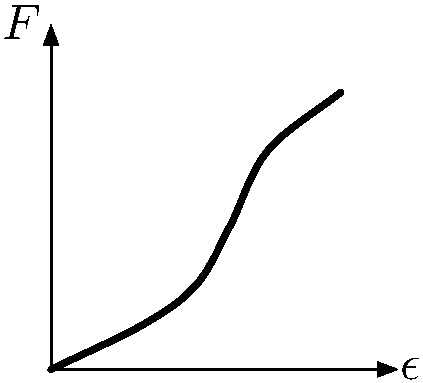
\includegraphics[width=4cm]{forcelong}
\caption{Articulations élastiques : force de rappel en fonction de l'élongation}
\label{Fig:forcelong}
\end{center}
\end{figure}
Souvent, pour des raisons de simplicité, on adopte un modèle linéaire c-à-d:
\begin{align*}
F_1 &= k_0(\tilde x_2 - \tilde x_1) = k_0((x_2 - x_1) - (d_1\cos\theta_1 + d_2\cos\theta_2)), \\
F_2 &= k_0(\tilde y_2 - \tilde y_1) = k_0((y_2 - y_1) - (d_1\sin\theta_1 + d_2\sin\theta_2)),
\end{align*}
où la constante $k_0$ est appelée {\em constante de rappel} du ressort. Dans ce cas, les 
équations du mouvement (\ref{eqmou1})-(\ref{eqmou6}) se réécrivent comme suit:
\begin{align*}
m_1\ddot x_1 &= k_0((x_2 - x_1) - (d_1\cos\theta_1 + d_2\cos\theta_2)), \\
m_1\ddot y_1 &= k_0((y_2 - y_1) - (d_1\sin\theta_1 + d_2\sin\theta_2)), \\
I_1\ddot \theta_1 &= k_0d_1((x_1 - x_2  + d_1\cos\theta_1 + d_2\cos\theta_2)\sin\theta_1 \\
&\hd +  (y_2 -y_1  - d_1\sin\theta_1 - d_2\sin\theta_2)\cos\theta_1), \\
m_2\ddot x_2 &= - k_0((x_2 - x_1) - (d_1\cos\theta_1 + d_2\cos\theta_2)), \\
m_2\ddot y_2 &= - k_0((y_2 - y_1) - (d_1\sin\theta_1 + d_2\sin\theta_2)), \\
I_2\ddot \theta_2 &=  k_0d_2((x_2 - x_1 - d_1\cos\theta_1 - d_2\cos\theta_2)\sin\theta_2 \\
&\hd +  (y_1 -y_2 + d_1\sin\theta_1 + d_2\sin\theta_2)\cos\theta_2). \qed
\end{align*}
\end{exemple}

Cet exemple montre que dans le cas d'un système mécanique articulé, le modèle dynamique 
général (\ref{modmecgen}) est modifié comme suit :
\eqn
M(q)\ddot{q} + f(q,\dot{q}) + g(q) + k(q) = G(q)u \label{modgenflex}
\eeqn
où apparaît le terme additionnel $k(q)$ qui représente l'effet des forces de rappel
du à la présence d'articulations élastiques dans le système.

\section{Frottement}
\markboth{{\bf \hspace*{5mm}Chapitre 2 }\hfill Systèmes mécaniques articulés}
{{ \bf Sec. \thesection }\hfill Frottement\hspace*{5mm}} 

La présence de forces de frottement est un autre phénomène physique que nous avons 
négligé jusqu'ici et qui a souvent un effet important sur le mouvement 
des systèmes mécaniques. En particulier, dans le cas d'articulations élastiques
modélisées comme dans la section précédente, la présence d'un amortissement 
par le frottement est indispensable si l'on veut éviter de développer des modèles 
qui soient le siège d'oscillations persistantes peu conformes à la réalité 
expérimentale.

Il y a plusieurs manières d'introduire le frottement dans la description d'un système
mécanique articulé. Nous retiendrons ici la plus simple qui consiste à supposer
que le mouvement de chacune des coordonnées $q_i$ du vecteur des coordonnées 
généralisées $q = (q_1, q_2, \hdots , q_\delta)$ est affecté par une force de frottement
séparée ne dépendant que de la vitesse $(\dot{q_i})$ de cette même coordonnée et
notée $h_i(\dot{q_i})$. Le vecteur de ces forces de frottement est lui même noté
$$
h(\dot{q}) = \bma{c} h_1(\dot{q_1}) \\ h_2(\dot{q_2}) \\ \vdots \\ h_{\delta}(\dot{q_\delta}) \ema
$$
de sorte que le modèle dynamique général (\ref{modgenflex}) est augmenté comme suit :
$$
M(q)\ddot{q} + f(q,\dot q) + g(q) + k(q) + h(\dot{q}) = G(q)u. \label{modgenflexfrot}
$$
La forme la plus courante des fonctions $h_i(\dot q_i)$ est la suivante :
$$
h_i(\dot q_i) = \alpha_{i}\mbox{sign}(\dot q_i) + \beta_i(\dot q_i).
$$
Dans cette équation le premier terme $\alpha_{i}\mbox{sign}(\dot q_i)$ représente le frottement
sec tandis que le deuxième terme $\beta_i(\dot q_i)$ représente le frottement
visqueux. Le coefficient $\alpha_i$ est constant. La fonction $\beta_i$ est monotone croissante avec $\beta(0) = 0$. On remarquera que la fonction $h$ est discontinue à l'origine, ce
qui peut entrainer des difficultés pour la simulation et l'analyse du système. Dans les applications qui seront considérées dans ce livre, sauf indication contraire, nous supposerons que le frottement sec est négligé ($\alpha_i = 0$).

\section{Energie et équation d'Euler-Lagrange} 

L'énergie cinétique $E_C$ d'un système mécanique articulé est définie comme suit~:
$$
E_C(q,\dot q) =  \frac{1}{2} \dot q^T M(q) \dot q.
$$
L'énergie potentielle $E_P$ est une primitive de la somme des forces dérivant d'un
potentiel, c'est à dire les forces de gravité et les forces de rappel des ressorts~:
$$
\frac{\partial E_P(q)}{\partial q} = g^T(q) + k^T(q).
$$
L'énergie totale $E_T$ est la somme de l'énergie cinétique et de l'énergie potentielle :
$$
E_T = E_C + E_P.
$$
L'évolution de l'énergie totale au cours du mouvement du système est examinée en
calculant sa dérivée temporelle :
\begin{equation} \begin{split}
\dot E_T &= \frac{\partial E_C}{\partial \dot q}\ddot q + \frac{\partial E_C}{\partial q}\dot q
+ \frac{\partial E_P}{\partial q}\dot q \\
&= \dot q^T [M(q) \ddot q + \frac{1}{2} \dot M(q) \dot q + g(q) + k(q)].
\end{split} \end{equation}
En substituant l'expression de $M(q)\ddot q$ extraite de l'équation générale du mouvement
(\ref{eqmouv}), on obtient :
$$
\dot E_T = \frac{1}{2} \dot q^T [\dot M(q) - 2C(q,\dot q)] \dot q + \dot q^T [G(q)u - h(\dot q)].
$$
Le premier terme du membre de droite de cette équation est nul car la matrice $\dot M(q) - 2C(q,\dot q)$
est antisymétrique (voir plus haut). Il reste donc :
$$
\dot E_T = \dot q^T [G(q)u - h(\dot q)].
$$
Lorsque le système n'est soumis à aucune autre force que celles qui dérivent d'un
potentiel, l'énergie totale est constante tout au long du mouvement :
$$
G(q)u - h(\dot q) = 0 \hspace{5mm} \Rightarrow \hspace{5mm} \dot E_T = 0.
$$
Dans ce cas, on dit que le système est {\em conservatif}.

En utilisant les propriétés (\ref{prop1}) et (\ref{prop2}), on vérifie aussi que l'énergie
cinétique satisfait la relation suivante :
\eqnn
\frac{d}{dt}(\frac{\partial E_C}{\partial \dot q})^T - (\frac{\partial E_C}{\partial q})^T = 
M(q)  \ddot q + C(q, \dot q) \dot q.
\eeqnn
Il s'en suit qu'une expression alternative de l'équation générale du mouvement (\ref{eqmouv})
est donnée par l'expression :
\eqnn
\frac{d}{dt} (\frac{\partial L(q, \dot q)}{\partial \dot q})^T - (\frac{\partial L(q, \dot q)}
{\partial q})^T = G(q)u - h(\dot q)
\eeqnn
avec :
\eqnn
L(q, \dot q) \triangleq E_C(q, \dot q) - E_P(q, \dot q).
\eeqnn
Cette équation porte généralement le nom d'{\em équation d'Euler-Lagrange} et la
quantité $L(q, \dot q)$ est appelée {\em Lagrangien} du système.

\section{Systèmes non-holonomes}

Les systèmes non-holonomes sont des systèmes mecaniques articulés dont
les contraintes de parcours peuvent dépendre non seulement des positions
$q$ mais aussi des vitesses $\dot q$. Lorsque ces contraintes ne
peuvent etre intégrées pour produire des contraintes de parcours qui
dépendent exclusivement des coordonnées de configuration, elles sont
appel\'ees {\it non-holonomes}. Cette situation se pr\'esente dans de
nombreuses applications pratiques, notamment dans le
domaine de l'automobile, dans le domaine a\'eronautique et en
robotique. Nous consid\'erons le cas particulier d'un
syst\`eme ayant $\delta$ degr\'es de libert\'e qui est soumis \`a
$m$ contraintes non-holonomes ind\'ependantes ($m < \delta$) qui sont  
lin\'eaires par rapport aux vitesses :
$$
N^T(q) \dot q = 0
$$
avec la matrice $N^T(q)$ de dimensions $(m \times \delta)$ et de plein rang.
Définissons la matrice $S(q)$, de dimensions $\delta \times (\delta - m)$ et de
plein rang, telle que :
\eqnn
N^T(q)S(q)=0.
\eeqnn
Les contraintes sont \'equivalentes au fait que le vecteur des vitesses
$\dot q$ appartient \`a l'espace engendr\'e par les colonnes de la matrice
$S(q)$ ou, autrement dit, qu'il existe un vecteur $\eta$ de dimension
$(\delta-m)$ tel que :
\eqn
\dot q = S(q) \eta. \label{modcin}
\eeqn
Les \'equations du mouvement s'\'ecrivent sous la forme standard :
\eqnn
M(q) \ddot{q} + f(q, \dot q) + g(q) + N(q)\lambda = G(q) u,
\eeqnn
en y ajoutant le terme $N(q)\lambda$ qui repr\'esente les forces de liaison
qui garantissent que les contraintes sont satisfaites le long du
mouvement (voir section 1.2.3). On \'elimine les multiplicateurs de
Lagrange $\lambda$ en pr\'emultipliant cette \'equation par $S^T(q)$:
\eqnn
S^T(q)M(q) \ddot{q} + S^T(q)[C(q, \dot q) \dot q + g(q)] = S^T(q)G(q)u.
\eeqnn
Finalement, en utilisant la relation (\ref{modcin}), on
obtient l'expression :
\eqn
J(q) \dot \eta + F(q, \eta) = S^T(q)G(q)u \label{moddyn}
\eeqn
avec
\eqnn
J(q) &=& S^T(q)M(q)S(q) \\
F(q, \eta) &=& S^T(q) M(q) \{ [\partial_q S(q)] S(q) \eta \} \eta +
S^T(q)f(q, S(q) \eta).
\eeqnn
Le mod\`ele dynamique g\'en\'eral d'un syst\`eme non-holonome est ainsi
constitu\'e
des \'equations (\ref{modcin}) et (\ref{moddyn}) que l'on peut \'ecrire sous
la forme d'un mod\`ele d'\'etat:
\eqnn
\dot q &=& S(q) \eta \\
\dot \eta &=& J^{-1}(q) [ -F(q, \eta) + S^T(q)G(q) u ].
\eeqnn
On observe que le vecteur d'\'etat :
\eqnn
\bma{c} q \\ \eta \ema
\eeqnn
est de dimension $(2\delta-m)$ avec les coordonn\'ees $\eta$ homog\`enes \`a
des vitesses. 

\section{Exercices}

\begin{exercice}{\bf \em Robots manipulateurs}

On a représenté à la figure \ref{Fig:exe-robot} trois configurations de robots
planaires à deux degrés de liberté.  Pour chacune de ces
configurations~:
\begin{enumerate}
\item Etablir le modèle dynamique du système et le modèle
d'état correspondant.  Expliciter les matrices $M(q), C(q,\dot q)$
et $G(q)$ ainsi que le vecteur $g(q)$.
\item Vérifier que le modèle est conservatif et qu'il satisfait l'équation
d'Euler-Lagrange.
\item Indiquer comment se modifient les équations du modèle si
les segments sont soumis à un frottement visqueux proportionnel au
carré de la vitesse. \qed
\end{enumerate}
\begin{figure}[ht]
\begin{center}
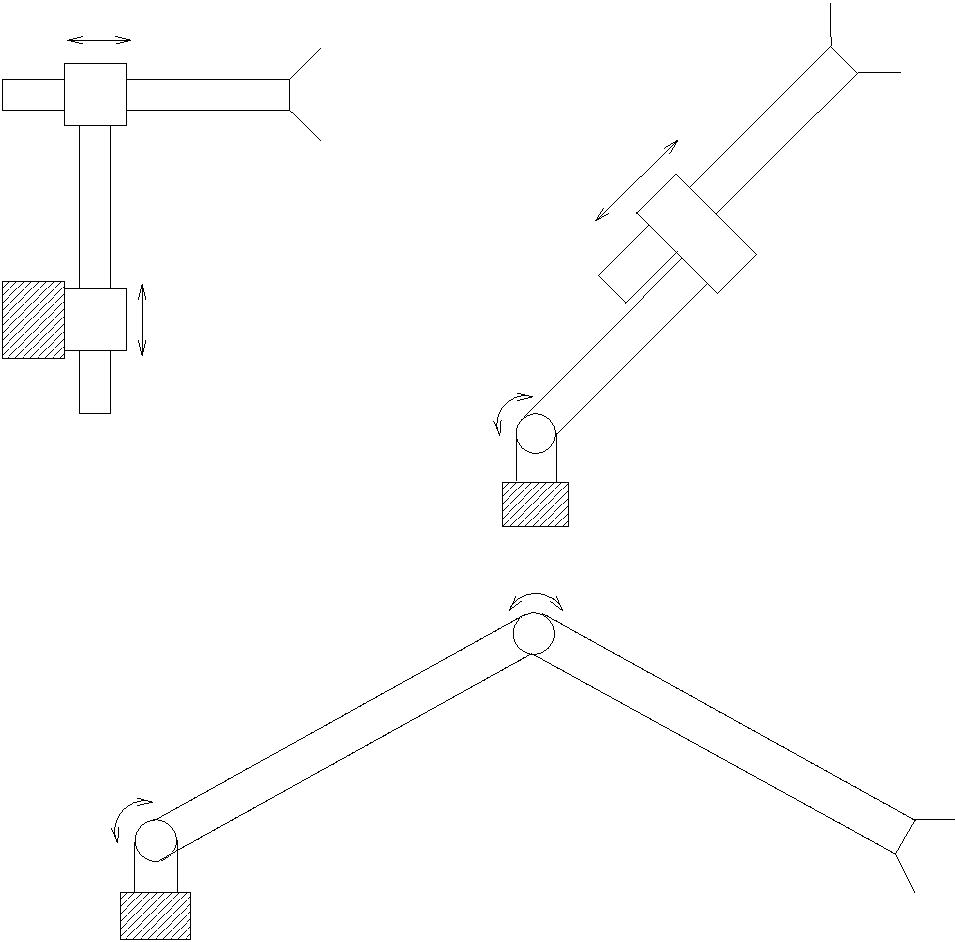
\includegraphics[width=3.5in]{exe-robot}
\caption{Configurations de robots manipulateurs planaires}
\label{Fig:exe-robot}
\end{center}
\end{figure}
\end{exercice}
\vv
\begin{figure}[!h]
\begin{center}
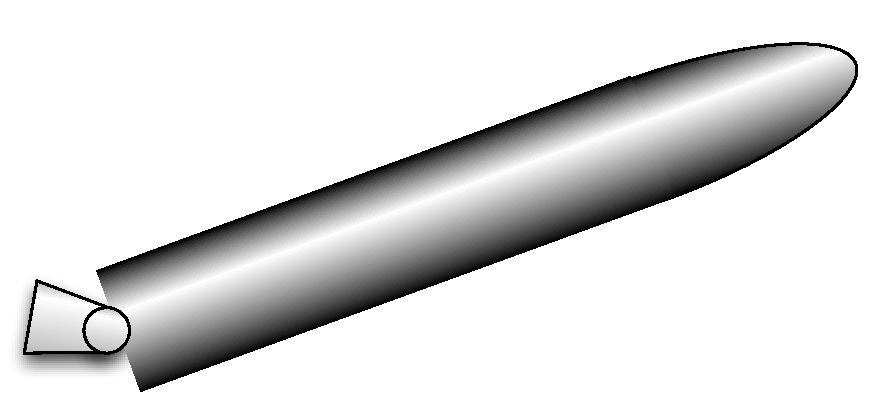
\includegraphics[width=8cm]{exe-fusee}
\caption{Fusée à moteur orientable}
\label{Fig:exe-fusee}
\end{center}
\end{figure}
\begin{exercice}{\bf \em Modélisation de la dynamique d'une fusée}

On considère une fusée propulsée par un moteur à réaction
orientable comme indiqué sur la figure \ref{Fig:exe-fusee} et se dépla\c
cant dans un plan vertical.  L'orientation du moteur est pilotée
par un actionneur hydraulique fournissant un couple $T$.  Le moteur
lui-même fournit une force de propulsion $F$.
\begin{enumerate}
\item Etablir les équations du modèle d'état du système,
sous l'hypothèse que les deux parties de la fusée (corps
principal et moteur) sont des corps rigides de masse constante. \qed
\end{enumerate}
\end{exercice}

\begin{exercice}{\bf \em Modélisation dynamique du module d'excursion
lunaire}

Lors de la mission Apollo 11, les astronautes Armstrong et Aldrin
se sont posés sur la lune au moyen du LEM (Lunar
Excursion Module; Fig. \ref{Fig:exe-lem}).  On considère les hypothèses de
modélisation suivantes :
\begin{figure}[ht]
\begin{center}
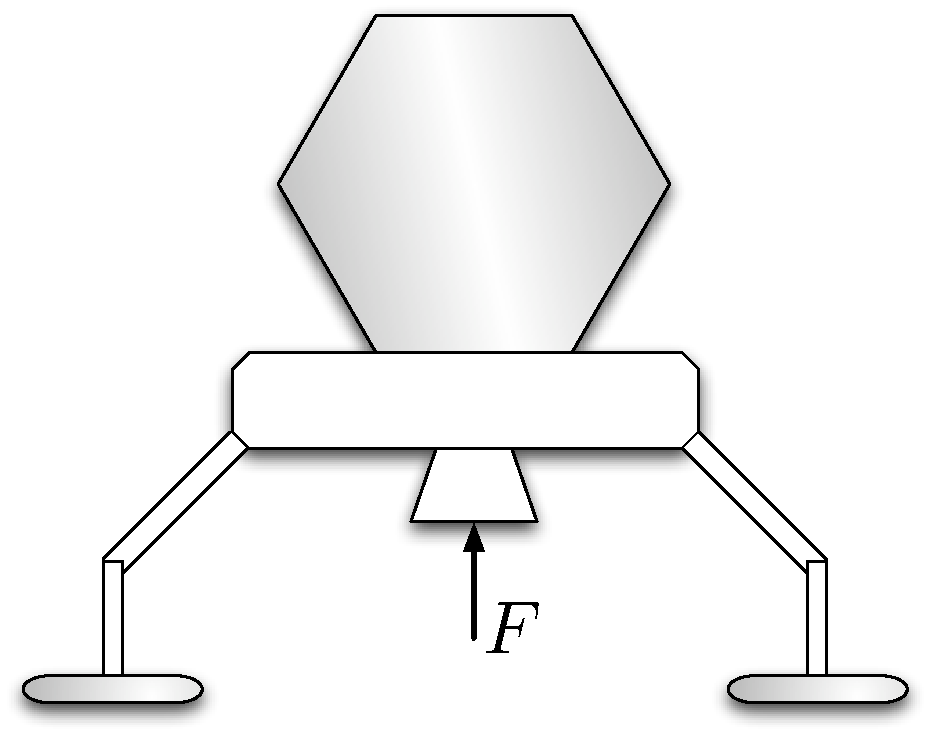
\includegraphics[width=2in]{exe-lem}
\caption{Module d'excursion lunaire}
\label{Fig:exe-lem}
\end{center}
\end{figure}
\begin{itemize}
\item[a)] le LEM est un corps rigide
\item[b)] le mouvement est vertical
\item[c)] les forces agissant sur le système sont la poussée $F$
et l'attraction lunaire
\item[d)] la masse de combustible embarqué constitue une partie
importante (non négligeable) de la masse totale du LEM
\item[e)] la masse de combustible consommée par unité de
temps est proportionnelle à $F$.
\end{itemize}
\begin{enumerate}
\item Etablir un modèle d'état du système qui satisfait ces
hypothèses de modélisation.
\item Quelles sont les principales limites de validité de ce
modèle ? \qed
\end{enumerate}
\end{exercice}
\vv

\begin{exercice}{\bf \em Un train pendulaire}

Un train pendulaire est un train qui peut se déplacer à
très grande vitesse dans les virages sans qu'il soit nécessaire
d'incliner les voies. 
\begin{figure}[ht]
\begin{center}
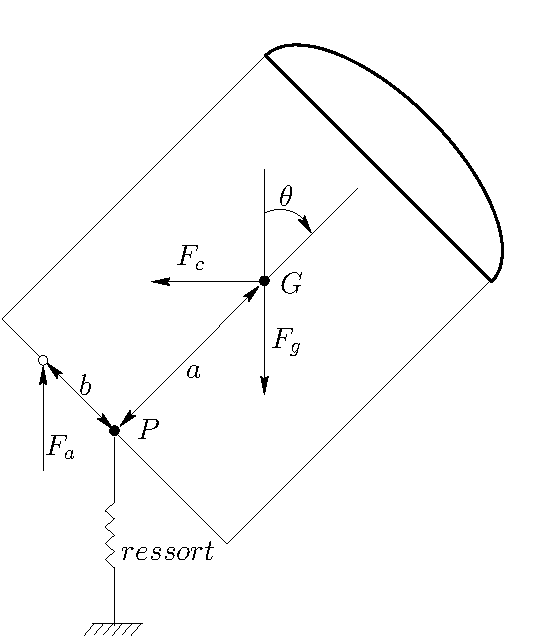
\includegraphics[width=7cm]{train2}
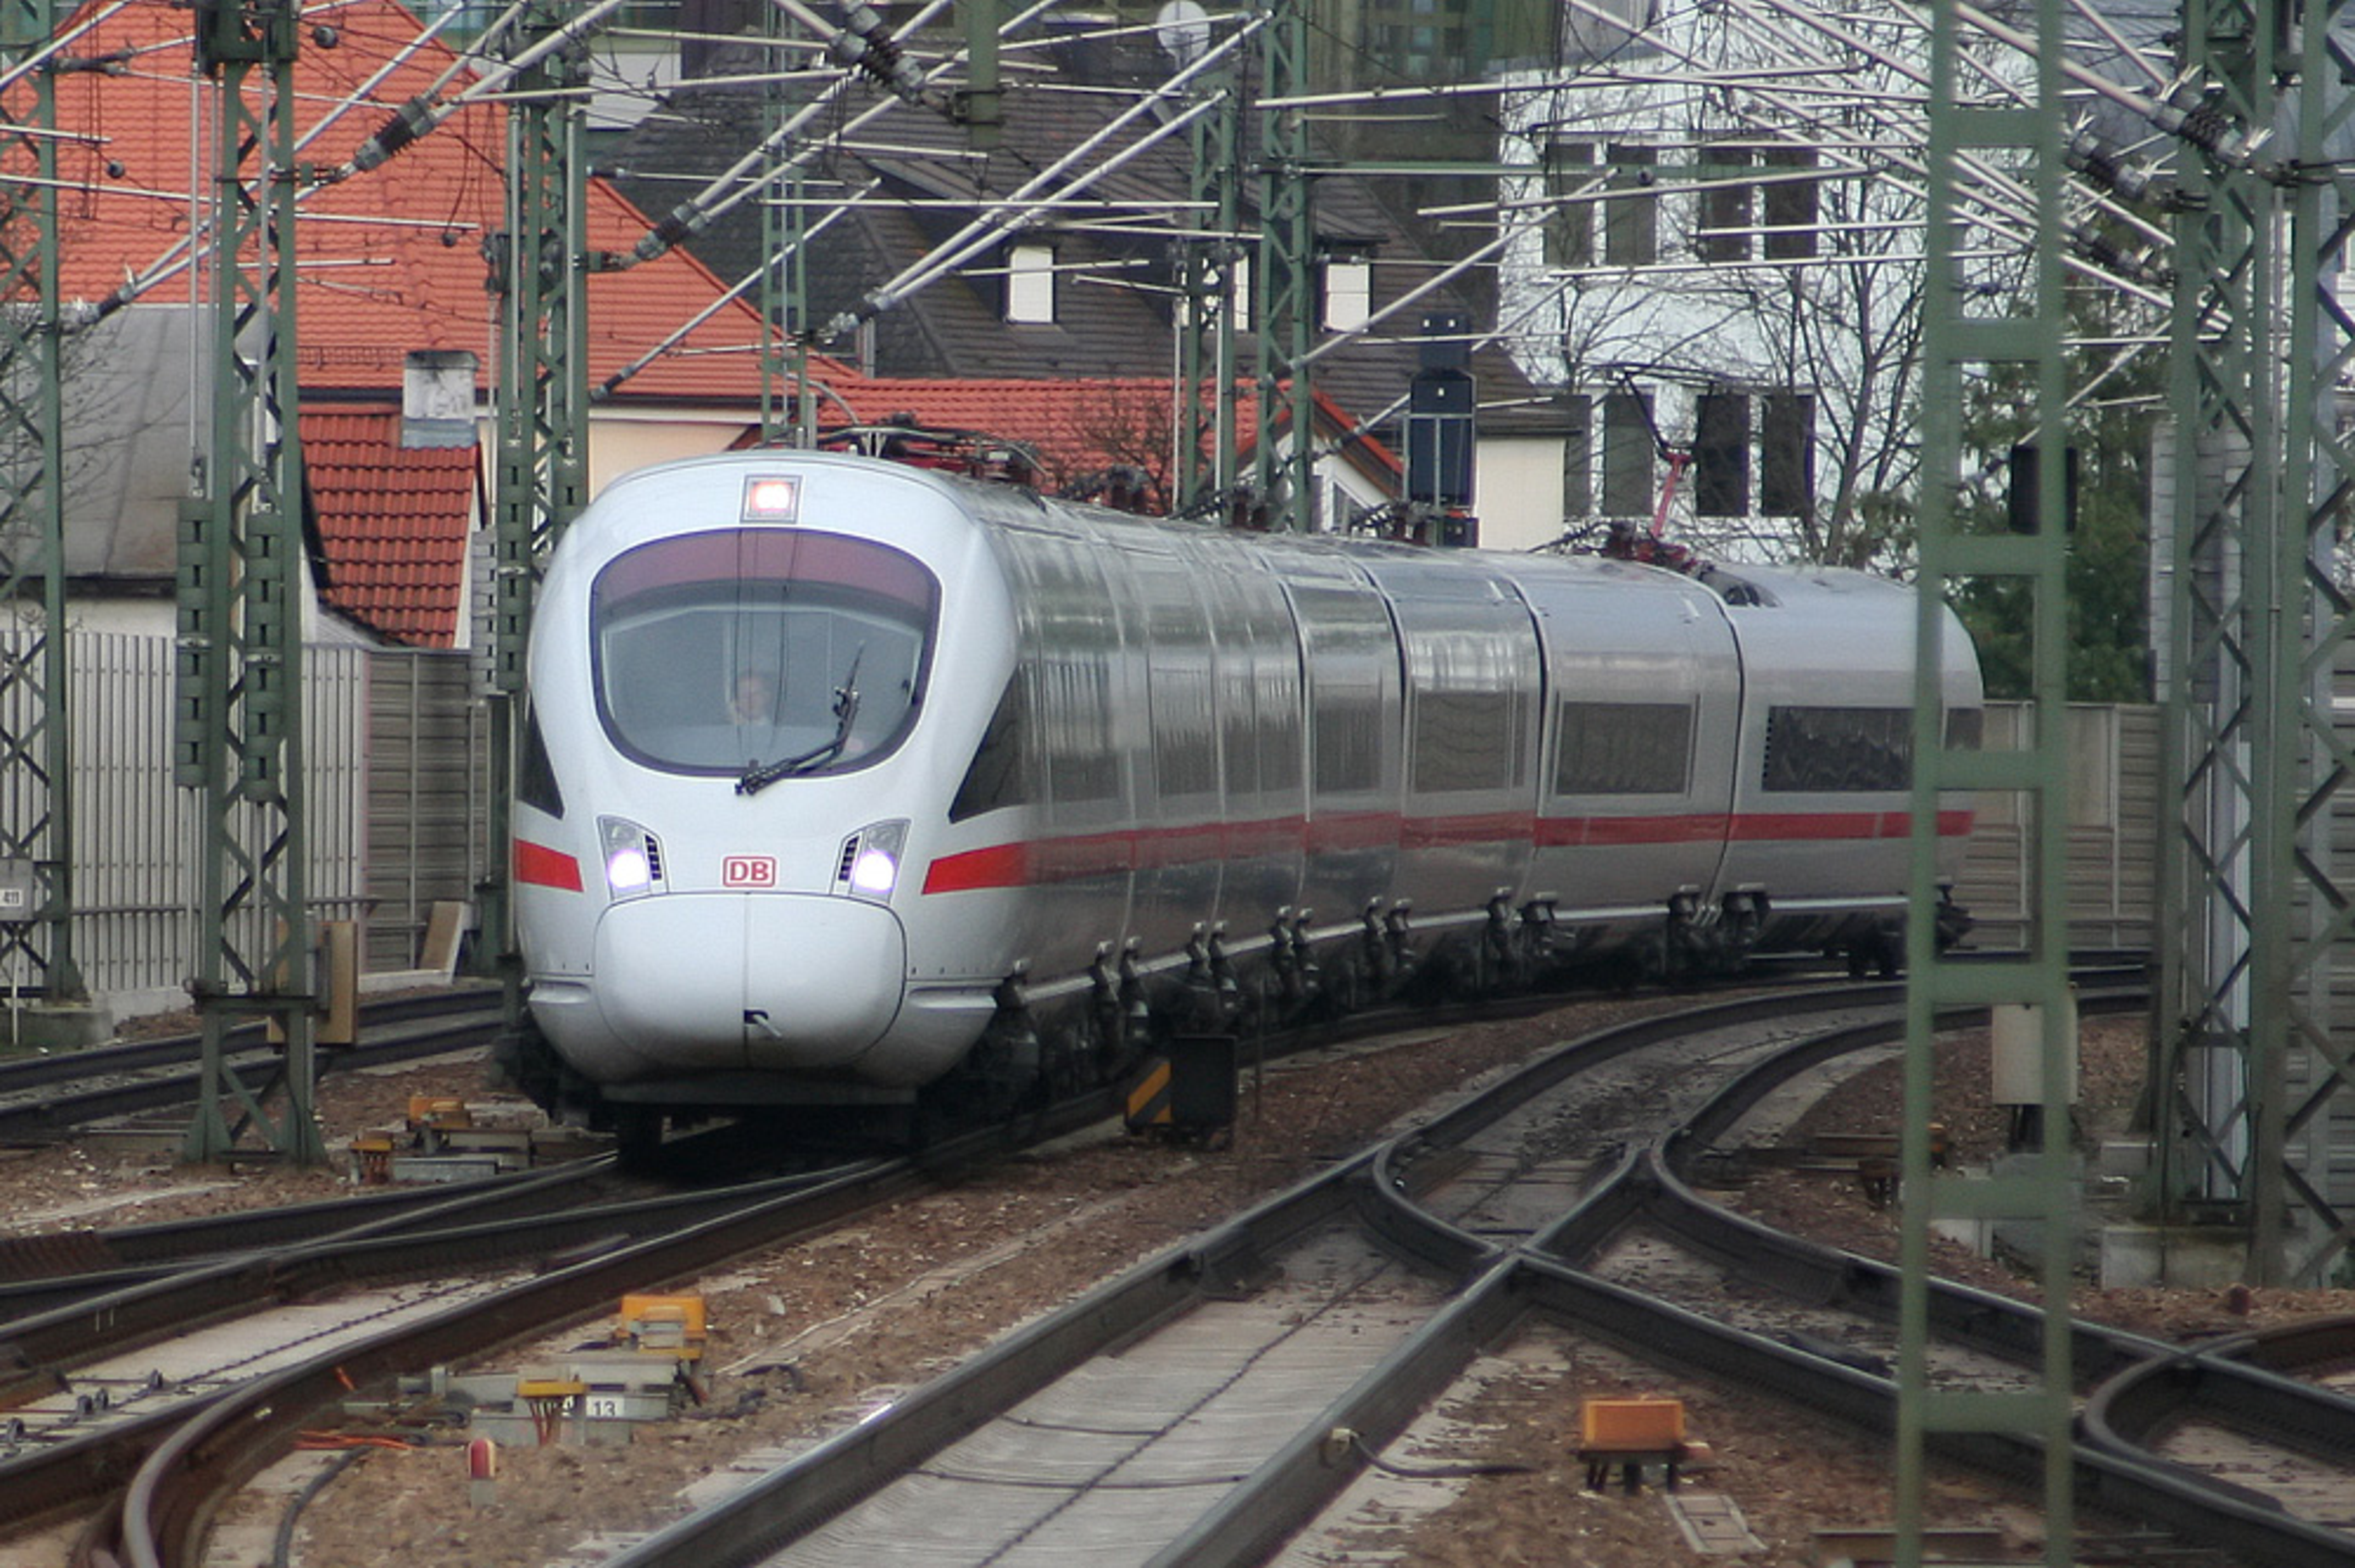
\includegraphics[width=5cm]{trainpendulaire}
\caption{Un train pendulaire}
\label{Fig:train}
\end{center}
\end{figure}
\begin{figure}[!h]
\begin{center}
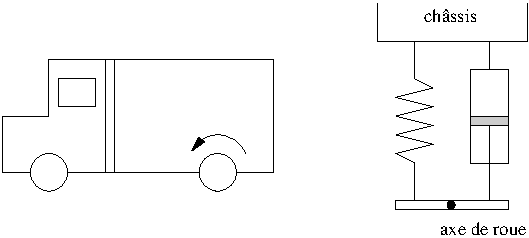
\includegraphics[width=3in]{exe-camion}
\caption{Modélisation de la dynamique d'un camion}
\label{Fig:exe-camion}
\end{center}
\end{figure}
Pour cela chaque voiture est munie d'un dispositif
actif qui applique une force verticale à la caisse de la voiture pour
contrebalancer l'effet de la force \og centrifuge \fg. Ceci est illustré sur
la figure \ref{Fig:train} où une section de la caisse d'une voiture est
représentée schématiquement avec $F_g$ la force de gravité
(appliquée au centre de masse $G$), $F_c$ la force "centrifuge" et
$F_a$ la force appliquée. On suppose que la ligne d'action de la force
$F_a$ est verticale quelle que soit la position angulaire $\theta$ de la
caisse. D'autre part la suspension de la voiture est schématisée par
un ressort vertical qui exerce une force proportionnelle à son
élongation. Le point d'application
$P$ du ressort est {\it contraint de se déplacer verticalement}.
Etablir un modèle d'état du système. \qed
\end{exercice}
\vv

\begin{exercice}{\bf \em Modélisation de la dynamique d'un camion}

On considère un camion se dépla\c cant en ligne droite (Fig. \ref{Fig:exe-camion}), sous les hypothèses de modélisation suivantes~:
\begin{itemize}
\item[a)] Le camion est un système articulé composé de corps rigides (caisse et
roues).
\item[b)] Le camion est équipé d'une propulsion arrière (le couple développé par
le moteur est transmis aux roues arrières).
\item[c)] Les roues roulent sans glisser.
\item[d)] Les roues sont reliées au chassis par un système de suspension composé
d'un ressort linéaire et d'un amortisseur à frottement visqueux de masse
négligeable.  Ce système de suspension ne permet que des déplacements verticaux.
\end{itemize}
\begin{enumerate}
\item Etablir un modèle d'état du système qui satisfait ces hypothèses de
modélisation (se limiter à deux corps : le chassis et une roue motrice).
\item Quelles sont les principales limites de validité de ce modèle ? \qed
\end{enumerate}
\end{exercice}
\vv

\begin{exercice}{\bf \em Un bateau}

Un bateau muni d'un moteur orientable de type \og hors-bord \gf se déplace sur un fleuve comme illustré à la figure \ref{bateau} (vue du dessus). Le fleuve est de largeur constante (= 2$L$). La poussée du moteur est représentée par le vecteur de longueur $F$ (= grandeur de la force de propulsion) et d'orientation $\beta$. Le bateau est aussi soumis à la force du courant du fleuve qui est une fonction parabolique de l'abscisse $y$ : le courant est nul aux deux bords et maximum au milieu du fleuve. Quand le moteur est à l'arrêt, le bateau est entraîné à la vitesse du courant par la force de frottement de l'eau sur la coque. 
\begin{enumerate}
\item Etablir un modèle d'état du système. Pour simplifier, on peut supposer que :
\begin{itemize}
\item[a)] le bateau est un corps rigide de masse constante;
\item[b)] le plan d'eau est quasi-horizontal et la gravité n'influence pas le mouvement du bateau;
\item[c)] la force exercée par le courant s'applique ponctuellement au centre de masse du bateau (on néglige le fait que la force du courant peut s'exercer de manière variable en divers points de la coque).
\end{itemize}
\item Quelle doit être la capacité de propulsion du moteur pour que l'on ait la garantie que le bateau pourra remonter le courant ? \qed
\end{enumerate} 
\begin{figure}[h]
\begin{center}
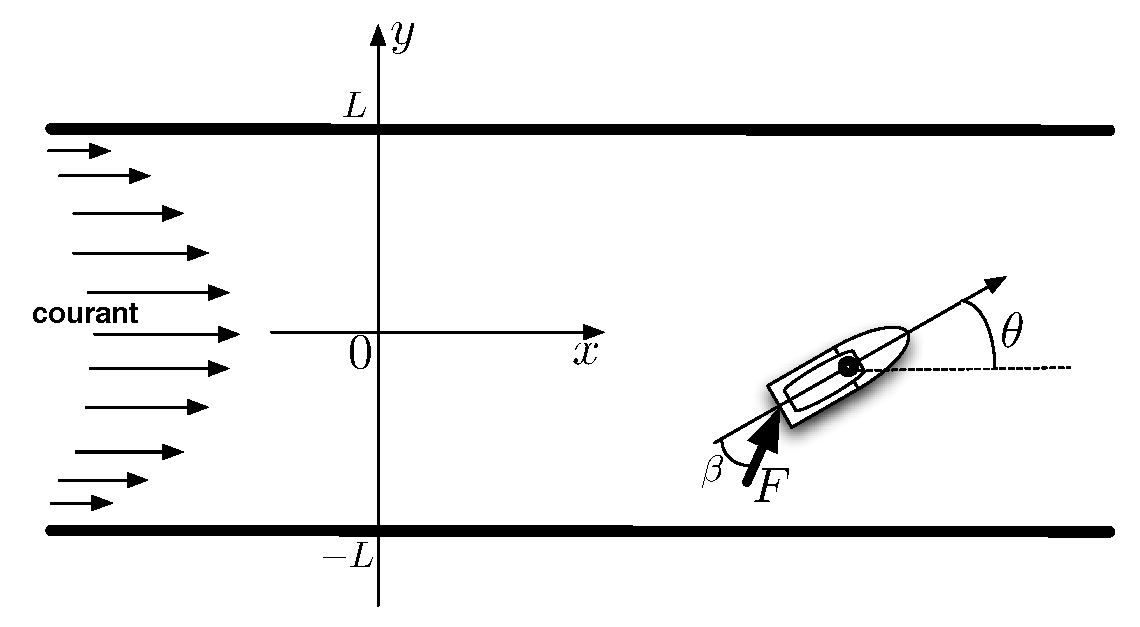
\includegraphics[width=10cm]{bateau}
\caption{Un bateau}
\label{bateau}
\end{center}
\end{figure}
\end{exercice}
\vv



\end{document}
